\chapter{Implementacija i korisničko sučelje}
		
		
		\section{Korištene tehnologije i alati}
			 
			 Komunikacija u timu realizirana je korištenjem aplikacije \underline{Discord}\footnote{https://discord.com/}. Za izradu UML dijagrama korišten je alat \underline{Astah Professional}\footnote{https://astah.net/products/astah-professional/}, a kao sustav za upravljanje izvornim kodom \underline{Git}\footnote{https://git-scm.com/}. Udaljeni repozitorij projekta je dostupan na web platformi \underline{GitHub}\footnote{https://github.com/}.
			 
			 Kao razvojno okruženje korišten je \underline{IntelliJ IDEA}\footnote{https://www.jetbrains.com/idea/} - integrirano je razvojno \newline okruženje (IDE) tvrtke JetBrains. Prvenstveno se koristi za razvoj računalnih programa za operacijski sustav Windows, kao i za web-stranice, web-aplikacije, web-usluge i mobilne aplikacije. IntelliJ IDEA za razvoj softvera koristi JetBrains platforme i tehnologije za olakšavanje procesa razvoja. To uključuje podršku za razvoj u raznim programskim jezicima(poput Java, Kotlin, Groovy i mnogih drugih), za Android razvoj, Spring Framework, Web development(\textit{frontend} i \textit{backend}) itd. Uz IntelliJ IDEA ponešto je korišten i \underline{Visual Studio Code}\footnote{https://code.visualstudio.com/}, ali uglavnom kao text editor te za pisanje \underline{docker}\footnote{https://www.docker.com/} deploy skripte. Docker predstavlja platformu kao uslugu(Paas) koja koristi virtualizaciju na razini OS-a za isporuku programa u spremnicima. Spremnici osiguravaju izolaciju procesa, mreže i datotečnog sustava.
			 
			 Aplikacija je napisana koristeći radni okvir \underline{Spring Framework}\footnote{https://spring.io/} i jezik \underline{Java}\footnote{https://www.java.com/en/} za izradu \textit{backenda} te \underline{React}\footnote{https://react.dev/} i jezik \underline{TypeScript}\footnote{https://www.typescriptlang.org/} za izradu \textit{frontenda}. React, također poznat kao React.js ili ReactJS, je biblioteka u JavaScriptu za izgradnju korisničkih sučelja. Održavana je od strane Facebooka. React se najčešće koristi kao osnova u razvoju web ili mobilnih aplikacija. Složene aplikacije u Reactu obično zahtijevaju korištenje dodatnih biblioteka za interakciju s API-jem. Programski jezik TypeScript je nadogradnja na JavaScript, a napravio ga je Microsoft. Radni okvir Spring Framework nadograđuje mogućnosti samog operativnog sustava. Radi se o posebnoj infrastrukturi koja programerima nudi gotova rješenja i funkcionalnosti da bi ubrzala i pojednostavila razvoj aplikacija svih vrsta i oblika.
			 
			 Baza podataka se nalazi na poslužitelju u oblaku \underline{Render}\footnote{https://render.com/}.	
			
			\eject
		
	
			\section{Ispitivanje programskog rješenja}

			\textbf{\textit{dio 2. revizije}}\\
			
			\textit{U ovom poglavlju je potrebno opisati provedbu ispitivanja implementiranih funkcionalnosti na razini komponenti i na razini cijelog sustava s prikazom odabranih ispitnih slučajeva. Studenti trebaju ispitati temeljnu funkcionalnost i rubne uvjete.}
			
			\subsection{Ispitivanje komponenti}
			\textit{Potrebno je provesti ispitivanje jedinica (engl. unit testing) nad razredima koji implementiraju temeljne funkcionalnosti. Razraditi \textbf{minimalno 6 ispitnih slučajeva} u kojima će se ispitati redovni slučajevi, rubni uvjeti te izazivanje pogreške (engl. exception throwing). Poželjno je stvoriti i ispitni slučaj koji koristi funkcionalnosti koje nisu implementirane. Potrebno je priložiti izvorni kôd svih ispitnih slučajeva te prikaz rezultata izvođenja ispita u razvojnom okruženju (prolaz/pad ispita). }
			
			\subsection{Ispitivanje sustava}
			
			Ispitivanje sustava proveli smo pomoću dodatka za preglednik
			\underline{Selenium IDE} \footnote{https://www.selenium.dev/documentation/ide/}
			te koristeći \underline{Selenium WebDriver}
			\footnote{https://www.selenium.dev/documentation/webdriver/} unutar JUnit
			testova.
			
			\text{Ispitivanje pomoću Selenium WebDrivera prikazana su na slikama * i *}
			\renewcommand{\lstlistingname}{Kod}
			\begin{lstlisting}[
				language=Java,
				frame=single,
				label={lst:testLoginGoodCreds},
				basicstyle = \small,
				tabsize=2,
				showspaces=false,
				showstringspaces=false,
				commentstyle = \color{red}, %% set comment color
				keywordstyle = \color{blue}, %% set keyword color
				stringstyle = \color{applegreen}, %% set string color
				rulecolor = \color{black},
				caption={Test testLoginGoodCreds},
				breaklines=true]
@Test
public void testLoginGoodCreds() {
	WebDriver driver = new ChromeDriver();
	System.setProperty(
	"webdriver.chrome.driver", 
	"C:\\Users\\akrkl\\AppData\\Local\\Microsoft\\WindowsApps\\chromedriver.exe"
	);
	driver.manage().timeouts().implicitlyWait(10, TimeUnit.SECONDS);

	driver.get("http://localhost:5173/login");

	WebElement element = driver.findElement(By.id("email"));
	element.sendKeys("testadmin");

	element = driver.findElement(By.id("lozinka"));
	element.sendKeys("123");

	driver.findElement(By.cssSelector("button[type='submit']")).click();

	WebDriverWait wait = new WebDriverWait(driver, Duration.ofSeconds(2));
	try {
	wait.until(
		ExpectedConditions.presenceOfElementLocated(By.id("searchBarByCategories"))
	);

	String redirectUrl = driver.getCurrentUrl();

	Assertions.assertEquals(
		"http://localhost:5173/", redirectUrl
	);
	}
	finally {
	driver.quit();
	}
}	
			\end{lstlisting}
			
			U Kodu \ref{lst:testLoginGoodCreds} testira se uspješan login korisnika. WebDriver otvara stranicu za login, pronalazi elemente za unos korisničkog imena i lozinke te unosi podatke. Nakon toga klikne na gumb za prijavu i čeka da se pojavi element za pretraživanje po kategorijama. Na kraju provjerava je li korisnik preusmjeren na početnu stranicu. 
			
			\pagebreak
			
			\begin{lstlisting}[
				language=Java,
				frame=single,
				label={lst:testLoginBadCreds},
				basicstyle = \small,
				tabsize=2,
				showspaces=false,
				showstringspaces=false,
				commentstyle = \color{red}, %% set comment color
				keywordstyle = \color{blue}, %% set keyword color
				stringstyle = \color{applegreen}, %% set string color
				rulecolor = \color{black},
				caption={Test testLoginBadCreds},
				breaklines=true]
@Test
public void testLoginBadCreds() {
	WebDriver driver = new ChromeDriver();
	System.setProperty(
		"webdriver.chrome.driver",
		"C:\\Users\\akrkl\\AppData\\Local\\Microsoft\\WindowsApps\\chromedriver.exe"
	);
	driver.manage().timeouts().implicitlyWait(10, TimeUnit.SECONDS);
	driver.get("http://localhost:5173/login");

	WebElement element = driver.findElement(By.id("email"));
	element.sendKeys("testadmin");

	element = driver.findElement(By.id("lozinka"));
	element.sendKeys("wrongPassword");

	driver.findElement(By.cssSelector("button[type='submit']")).click();

	try {
		String redirectUrl = driver.getCurrentUrl();

		Assertions.assertNotEquals(
			"http://localhost:5173/", redirectUrl
		);
	}
	finally {
		driver.quit();
	}
}
			\end{lstlisting}
			
			U Kodu \ref{lst:testLoginBadCreds} testira se neuspješan login korisnika. WebDriver otvara stranicu za login, pronalazi elemente za unos korisničkog imena i lozinke te unosi podatke. Nakon toga klikne na gumb za prijavu i provjerava je li korisnik preusmjeren na početnu stranicu.
			
			\pagebreak
			
			\begin{figure}[!htb]
				\centering
				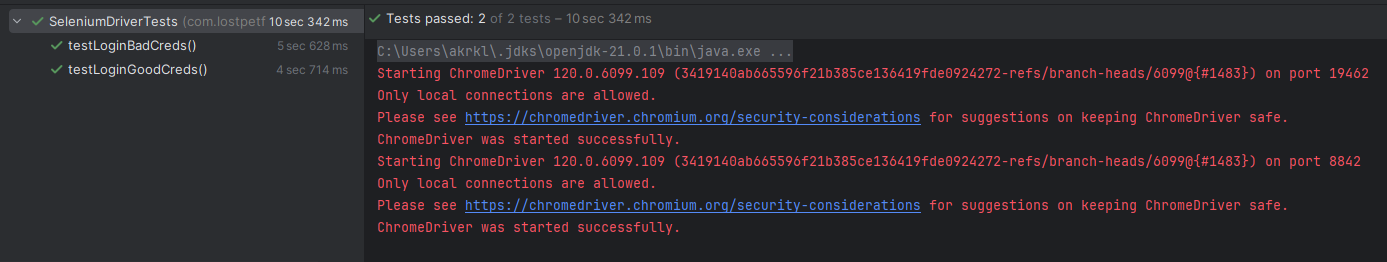
\includegraphics[width=\textwidth]{slike/test_passed.png}
				\caption{Testovi prolaze}
			\end{figure}
			
			\par\noindent\rule{\textwidth}{0.5pt}
			
			\begin{figure}[!htb]
				\centering
				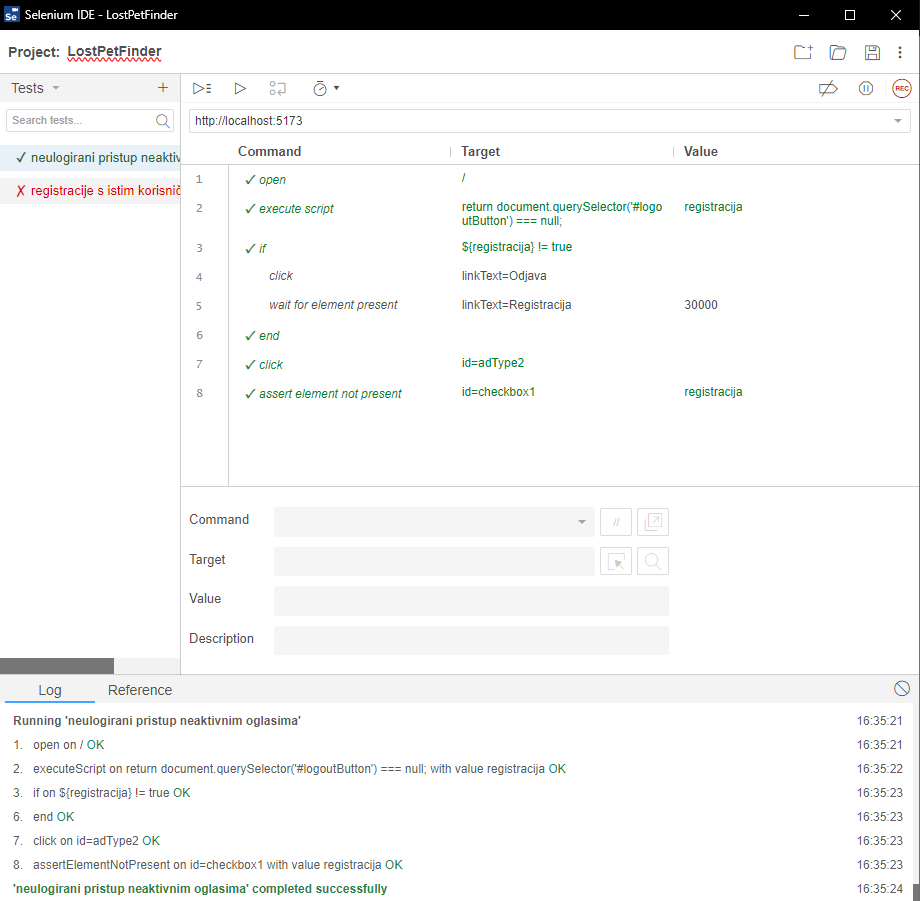
\includegraphics[width=\textwidth]{slike/selenium_test_1.png}
				\caption{Test: neulogirani korisnik pristupa neaktivnim oglasima}
			\end{figure}
			
			U ovom testu pomoću Selenium IDE-a provjerava se može li neulogirani korisnik pristupiti neaktivnim oglasima klikom na pripadajući radio button. Prvo se provjerava je li korisnik ulogiran, u tom slučaju se odjavljuje. Nakon toga se otvara stranica za prikaz oglasa, klikne se na radio button za prikaz neaktivnih oglasa i provjerava se je li se pojavio checkbox za filtriranje neaktivnih oglasa. Ako nije, test prolazi. Iz priloženog se vidi da aplikacija prolazi test.  
			
			\par\noindent\rule{\textwidth}{0.5pt}
			
			\begin{figure}[!htb]
				\centering
				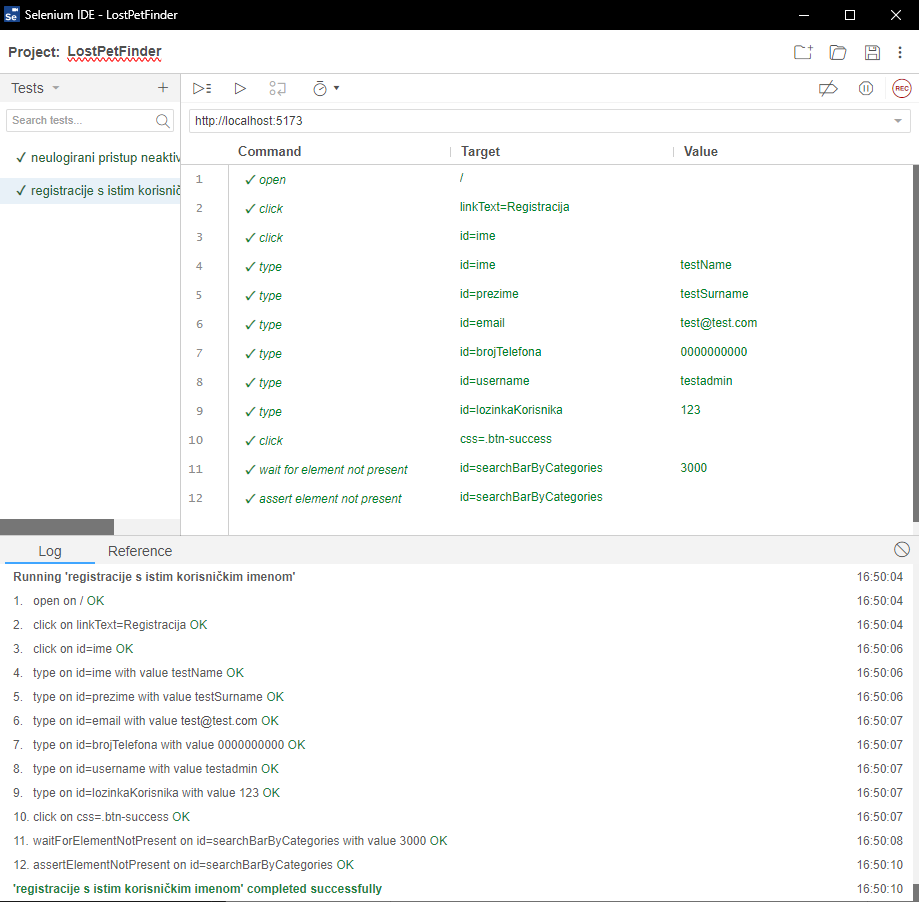
\includegraphics[width=\textwidth]{slike/selenium_test_2.png}
				\caption{Test: registracija s već postojećim podacima korisnika}
			\end{figure}
			
			U ovom testu pomoću Selenium IDE-a provjerava se kako aplikacija reagira na pokušaj registracije korisnika s podacima već postojećeg korisnika. Nakon unosa klikne se na gumb koji šalje formu i provjerava se je li se pojavio element za pretraživanje po kategorijama, odnosno je li se dogodio redirect na početnu stranicu. Ako nije, registracija nije uspjela i test prolazi. Iz priloženog se vidi da aplikacija prolazi test. 
			
			\eject
		
		
		\section{Dijagram razmještaja}
			
                \noindent Dijagrami razmještaja opisuju kako su komponente sustava raspoređene unutar njihovog radnog okruženja, uključujući sklopovlje i softversku podršku. Na poslužiteljskom računalu nalaze se web poslužitelj i poslužitelj baze podataka. Klijenti pristupaju web aplikaciji putem web preglednika. Arhitektura sustava temelji se na modelu "klijent-poslužitelj", gdje se komunikacija između računala korisnika (korisnik, registrirani korisnik, sklonište za životinje) i poslužitelja odvija preko HTTP veze.

                \begin{figure}[!htb]
		      \centering
		    \includegraphics[width=\textwidth]{slike/Dijagram_razmještaja}
		      \caption{Dijagram razmještaja}
		      \end{figure}
        
			\eject 
		
		\section{Upute za puštanje u pogon}
		
			\textbf{\textit{dio 2. revizije}}\\
		
			 \textit{U ovom poglavlju potrebno je dati upute za puštanje u pogon (engl. deployment) ostvarene aplikacije. Na primjer, za web aplikacije, opisati postupak kojim se od izvornog kôda dolazi do potpuno postavljene baze podataka i poslužitelja koji odgovara na upite korisnika. Za mobilnu aplikaciju, postupak kojim se aplikacija izgradi, te postavi na neku od trgovina. Za stolnu (engl. desktop) aplikaciju, postupak kojim se aplikacija instalira na računalo. Ukoliko mobilne i stolne aplikacije komuniciraju s poslužiteljem i/ili bazom podataka, opisati i postupak njihovog postavljanja. Pri izradi uputa preporučuje se \textbf{naglasiti korake instalacije uporabom natuknica} te koristiti što je više moguće \textbf{slike ekrana} (engl. screenshots) kako bi upute bile jasne i jednostavne za slijediti.}
			
			
			 \textit{Dovršenu aplikaciju potrebno je pokrenuti na javno dostupnom poslužitelju. Studentima se preporuča korištenje neke od sljedećih besplatnih usluga: \href{https://aws.amazon.com/}{Amazon AWS}, \href{https://azure.microsoft.com/en-us/}{Microsoft Azure} ili \href{https://www.heroku.com/}{Heroku}. Mobilne aplikacije trebaju biti objavljene na F-Droid, Google Play ili Amazon App trgovini.}
			
			
			\eject 